\documentclass[margin=5mm, tikz]{standalone}
\usepackage[utf8x]{inputenc}
\usepackage{pgfplots}
\pgfplotsset{compat=1.18}
\usepackage{tikz}
\usepackage{siunitx}
\usepackage{physics}

\begin{document}
    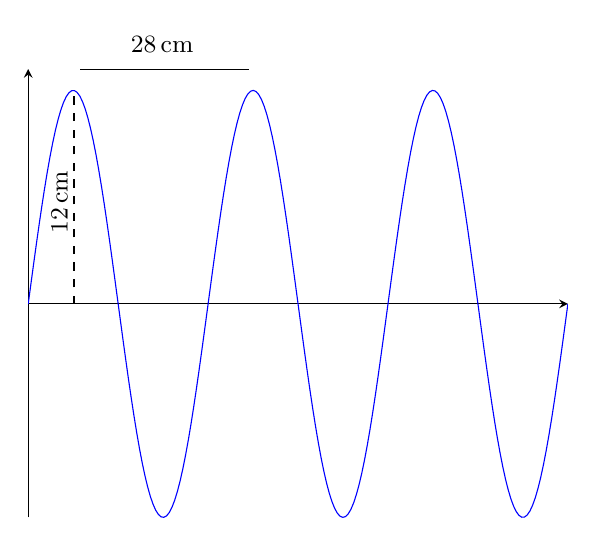
\begin{tikzpicture}
        \begin{axis}[
            domain=0:6*pi,
            samples=200,
            no marks,
            axis lines=middle,
            ticks=none
            ]

            \addplot {sin(deg(x))};
            \addplot[mark=none, dashed] coordinates {(1.6, 0) (1.6, 1)};
            \addplot[mark=none] coordinates {(1.8, 1.1) (7.7, 1.1)};
            % \node at (1.8, 5) {\small{$\SI{12}{\centi\meter}$}};
        \end{axis}
        \node [rotate=90] at (0.4, 4) {\small{$\SI{12}{\centi\meter}$}};
        \node at (1.7, 6) {\small{$\SI{28}{\centi\meter}$}};
    \end{tikzpicture}

\end{document}